 \documentclass[12pt]{amsart}
% packages
\usepackage{graphicx}
\usepackage{setspace}
\usepackage{amssymb,amsmath,amsthm,amsfonts,amscd}
\usepackage{hyperref}
\usepackage{color}
\usepackage{booktabs}
\usepackage{tabularx}
\usepackage{enumitem}
\usepackage[retainorgcmds]{IEEEtrantools}
\usepackage[notref,notcite,final]{showkeys}
\usepackage[final]{pdfpages}
\usepackage{fancyhdr}
\usepackage{upgreek}
\usepackage{multicol}

\usepackage{fancyvrb}
\usepackage{listings}
% set margin as 0.75in
\usepackage[margin=0.75in]{geometry}

% tikz-related settings
\usepackage{tikz}
\usepackage{tikz-cd}
\usetikzlibrary{cd}

% theorem environments with italic font
\newtheorem{thm}{Theorem}[section]
\newtheorem*{thm*}{Theorem}
\newtheorem{lemma}[thm]{Lemma}
\newtheorem{prop}[thm]{Proposition}
\newtheorem{claim}[thm]{Claim}
\newtheorem{corollary}[thm]{Corollary}
\newtheorem{conjecture}[thm]{Conjecture}
\newtheorem{question}[thm]{Question}
\newtheorem{procedure}[thm]{Procedure}
\newtheorem{assumption}[thm]{Assumption}

% theorem environments with roman font (use lower-case version in body
% of text, e.g., \begin{example} rather than \begin{Example})
\newtheorem{Definition}[thm]{Definition}
\newenvironment{definition}
{\begin{Definition}\rm}{\end{Definition}}
\newtheorem{Example}[thm]{Example}
\newenvironment{example}
{\begin{Example}\rm}{\end{Example}}

\theoremstyle{definition}
\newtheorem{remark}[thm]{\textbf{Remark}}

% special sets
\newcommand{\A}{\mathbb{A}}
\newcommand{\C}{\mathbb{C}}
\newcommand{\F}{\mathbb{F}}
\newcommand{\N}{\mathbb{N}}
\newcommand{\Q}{\mathbb{Q}}
\newcommand{\R}{\mathbb{R}}
\newcommand{\Z}{\mathbb{Z}}
\newcommand{\cals}{\mathcal{S}}
\newcommand{\ZZ}{\mathbb{Z}_{\ge 0}}
\newcommand{\cala}{\mathcal{A}}
\newcommand{\calb}{\mathcal{B}}
\newcommand{\cald}{\mathcal{D}}
\newcommand{\calh}{\mathcal{H}}
\newcommand{\call}{\mathcal{L}}
\newcommand{\calr}{\mathcal{R}}
\newcommand{\la}{\mathbf{a}}
\newcommand{\lgl}{\mathfrak{gl}}
\newcommand{\lsl}{\mathfrak{sl}}
\newcommand{\lieg}{\mathfrak{g}}

% math operators
\DeclareMathOperator{\kernel}{\mathrm{ker}}
\DeclareMathOperator{\image}{\mathrm{im}}
\DeclareMathOperator{\rad}{\mathrm{rad}}
\DeclareMathOperator{\id}{\mathrm{id}}
\DeclareMathOperator{\hum}{[\mathrm{Hum}]}
\DeclareMathOperator{\eh}{[\mathrm{EH}]}
\DeclareMathOperator{\lcm}{\mathrm{lcm}}
\DeclareMathOperator{\Aut}{\mathrm{Aut}}
\DeclareMathOperator{\Inn}{\mathrm{Inn}}
\DeclareMathOperator{\Out}{\mathrm{Out}}
\DeclareMathOperator{\Gal}{\mathrm{Gal}}


% frequently used shorthands
\newcommand{\ra}{\rightarrow}
\newcommand{\se}{\subseteq}
\newcommand{\ip}[1]{\langle#1\rangle}
\newcommand{\dual}{^*}
\newcommand{\inverse}{^{-1}}
\newcommand{\norm}[2]{\|#1\|_{#2}}
\newcommand{\abs}[1]{\lvert #1 \rvert}
\newcommand{\Abs}[1]{\bigg| #1 \bigg|}
\newcommand\bm[1]{\begin{bmatrix}#1\end{bmatrix}}
\newcommand{\op}{\text{op}}

% nicer looking empty set
\let\oldemptyset\emptyset
\let\emptyset\varnothing

\setlist[enumerate,1]{topsep=1em,leftmargin=1.8em, itemsep=0.5em, label=\textup{(}\arabic*\textup{)}}
\setlist[enumerate,2]{topsep=0.5em,leftmargin=3em, itemsep=0.3em}

%pagestyle
%\pagestyle{fancy} 

\begin{document}
\begin{center}
    \textsc{Random Walks. HW 4\\ Ian Jorquera\\ Collaboration: Tristan, Alex}
\end{center}
\vspace{1em}


\definecolor{codegreen}{rgb}{0,0.6,0}
\definecolor{codegray}{rgb}{0.5,0.5,0.5}
\definecolor{codepurple}{rgb}{0.58,0,0.82}
\definecolor{backcolour}{rgb}{1,1,1}

\lstdefinestyle{mystyle}{
    backgroundcolor=\color{backcolour},   
    commentstyle=\color{codegray},
    keywordstyle=\color{magenta},
    numberstyle=\tiny\color{codegray},
    stringstyle=\color{codegreen},
    basicstyle=\ttfamily\footnotesize,
    breakatwhitespace=false,         
    breaklines=true,                 
    captionpos=b,                    
    keepspaces=true,                 
    numbers=left,                    
    numbersep=5pt,                  
    showspaces=false,                
    showstringspaces=false,
    showtabs=false,                  
    tabsize=2
}

\lstset{style=mystyle}


\begin{enumerate}
    \item First we can construct the Markov chain which will be

    \begin{center}
            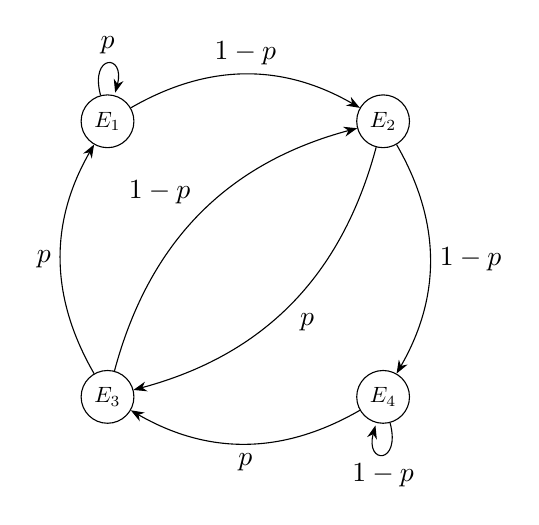
\begin{tikzpicture}
    
        % Add or remove nodes here, use the tuple for location
        \begin{scope}[every node/.style={circle,draw,scale=.8}]
        \node (A) at (0,3.5) {$E_1$};
        \node (B) at (3.5,3.5) {$E_2$};
        \node (C) at (0,0) {$E_3$};
        \node (D) at (3.5,0) {$E_4$};
        \end{scope}
    
        % forward(red)
        % Remove or add new edges here
        \begin{scope}[>={Stealth[black]},
                  every edge/.style={draw=black, thin}]. % you can change the color of the edges here
        \path [->] (A) edge[loop above, "$p$"] (A);
        \path [->] (A) edge[bend left, above, "$1-p$"] (B);
        
        \path [->] (B) edge[bend left, above, "$p$"] (C);
        \path [->] (B) edge[bend left, above, "$1-p$"] (D);
        
        \path [->] (C) edge[bend left, above, "$p$"] (A);
        \path [->] (C) edge[bend left, above, "$1-p$"] (B);
        
        \path [->] (D) edge[bend left, "$p$"] (C);
        \path [->] (D) edge[loop below, "$1-p$"] (D);
        \end{scope}
    
        \end{tikzpicture}
        \end{center}

Which has the transition matrix 
$$A=\begin{pmatrix}
    p & 0 & p & 0\\
    1-p & 0 & 1-p & 0\\
    0 & p & 0 & p\\
    0 & 1-p & 0 & 1-p\\
\end{pmatrix}$$

The square of this is 
$$A=\begin{pmatrix}
    p^2 & p^2 & p^2 & p^2 \\
    p(1-p) & p(1-p) & p(1-p) & p(1-p) \\
    p(1-p) & p(1-p) & p(1-p) & p(1-p) \\
    (1-p)^2 & (1-p)^2 & (1-p)^2 & (1-p)^2
\end{pmatrix}$$

\item In this situation we have the following Markov chain with all arrows on the top having probability of $\frac{1}{6}$
\begin{center}
            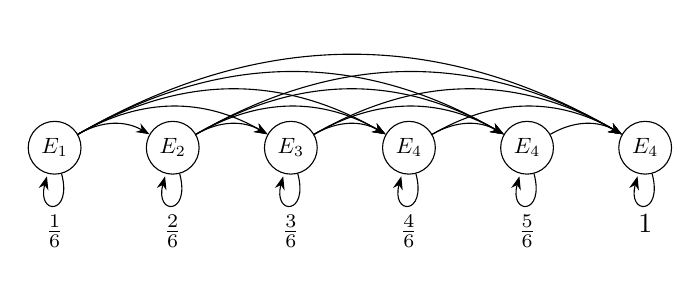
\begin{tikzpicture}
    
        % Add or remove nodes here, use the tuple for location
        \begin{scope}[every node/.style={circle,draw,scale=.8}]
        \node (A) at (0,0) {$E_1$};
        \node (B) at (1.5,0) {$E_2$};
        \node (C) at (3,0) {$E_3$};
        \node (D) at (4.5,0) {$E_4$};
        \node (E) at (6,0) {$E_4$};
        \node (F) at (7.5,0) {$E_4$};
        \end{scope}
    
        % forward(red)
        % Remove or add new edges here
        \begin{scope}[>={Stealth[black]},
                  every edge/.style={draw=black, thin}]. % you can change the color of the edges here
        \path [->] (A) edge[loop below, "$\frac{1}{6}$"] (A);
        \path [->] (A) edge[bend left, above ] (B);
        \path [->] (A) edge[bend left, above ] (C);
        \path [->] (A) edge[bend left, above ] (D);
        \path [->] (A) edge[bend left, above ] (E);
        \path [->] (A) edge[bend left, above ] (F);

        \path [->] (B) edge[loop below, "$\frac{2}{6}$"] (B);
        \path [->] (B) edge[bend left, above] (C);
        \path [->] (B) edge[bend left, above] (D);
        \path [->] (B) edge[bend left, above] (E);
        \path [->] (B) edge[bend left, above] (F);

        \path [->] (C) edge[loop below, "$\frac{3}{6}$"] (C);
        \path [->] (C) edge[bend left, above] (D);
        \path [->] (C) edge[bend left, above] (E);
        \path [->] (C) edge[bend left, above] (F);

        \path [->] (D) edge[loop below, "$\frac{4}{6}$"] (D);
        \path [->] (D) edge[bend left, above] (E);
        \path [->] (D) edge[bend left, above] (F);

        \path [->] (E) edge[loop below, "$\frac{5}{6}$"] (E);
        \path [->] (E) edge[bend left, above] (F);

        \path [->] (F) edge[loop below, "$1$"] (F);
        \end{scope}
    
        \end{tikzpicture}
        \end{center}
    The corresponding transition matrix is
    $$A=\begin{pmatrix}
    {1}/{6} & 0 & 0 & 0 & 0 & 0\\
    {1}/{6} & {2}/{6} & 0 & 0 & 0 & 0\\
    {1}/{6} & {1}/{6} & {3}/{6} & 0 & 0 & 0\\
    {1}/{6} & {1}/{6} & {1}/{6} & {4}/{6} & 0 & 0\\
    {1}/{6} & {1}/{6} & {1}/{6} & {1}/{6} & {5}/{6} & 0\\
    {1}/{6} & {1}/{6} & {1}/{6} & {1}/{6} & {1}/{6} & 1\\
\end{pmatrix}$$

\item 
\begin{enumerate}[label=(\alph*)]
    \item Let $\psi(t)=\displaystyle{\frac{1}{\tau}\text{exp}(-t/\tau)}$. In this case we have that $\psi(s)=\frac{1}{\tau}\int_{0}^{\infty}e^{-st-\frac{t}{\tau}}dt=\frac{1}{s\tau+1}$. we know that $\phi(s)=\frac{s\psi(s)}{1-\psi(s)}=\frac{\frac{s}{s\tau+1}}{1-\frac{1}{s\tau+1}}=\frac{\frac{s}{s\tau+1}}{\frac{s\tau}{s\tau+1}}=\frac{1}{\tau}$. This means that $\phi(t)=\frac{1}{\tau}\delta(t)$. And so when considering the generalized master equation we have that 

\begin{align*}
    \frac{dp(r,t)}{dt}&=\int_{0}^{t}\phi(t-t')\left(-P(r,t')+\sum_{r'\in \Omega}p(r,r')P(r',t')\right) dt'\\
    &= \int_{0}^{t}\frac{1}{\tau}\delta(t-t')\left(-P(r,t')+\sum_{r'\in \Omega}p(r,r')P(r',t')\right) dt'\\
    &= \frac{1}{\tau}\left(-P(r,t)+\sum_{r'\in \Omega}p(r,r')P(r',t)\right) dt'
\end{align*}

Which is exactly the ordinary master equation for a random walk in discrete space $\Omega$.\\

\item We know that the memory kernel in Laplace domain is $sM(s)=\phi(s)$ meaning we know that $M(s)=\frac{1}{s\tau}$. And so with the inverse Laplace transform we have that $M(t)=\frac{1}{\tau}$ for $t\geq 0$.\\
\end{enumerate}

\item Let $\psi(t)=At^{-(1+\alpha)}$ for $\leq \alpha\leq$. In this case we will consider the survival probability $F(t)=\int_{t}^{\infty}\psi(t')dt'=A\frac{t^{-\alpha}}{\alpha}=\frac{A}{\alpha}t^{(1-\alpha)-1}$. In which case from the Tauberian Theorems we know that $F(s)=\frac{A}{\alpha}\Gamma(1-\alpha)s^{-1+\alpha}$. This gives us that $\psi(s)=s(\frac{1}{s}-F(s))=1-s\frac{A}{\alpha}\Gamma(1-\alpha)\frac{s^{\alpha}}{s}=1-\frac{A}{\alpha}\Gamma(1-\alpha)s^{\alpha}$. We then know that 
$$M(s)=\frac{\psi(s)}{1-\psi(s)}=\frac{1-\frac{A}{\alpha}\Gamma(1-\alpha)s^{\alpha}}{\frac{A}{\alpha}\Gamma(1-\alpha)s^{\alpha}}=\frac{\alpha}{A\Gamma(1-\alpha)s^{-\alpha}}-1$$
And by the Tauberian Theorem and the linearity of Laplace transforms we have that 
$$M(t)=\frac{\alpha}{A\Gamma(1-\alpha)\Gamma(\alpha)}t^{\alpha-1}-\delta(t)$$
And so for large $t$ asymptotics we have that $M(t)\sim t^{\alpha-1}$.\\

\item The generalized master equation is

$$\frac{dP(\textbf{r},t)}{dt}=\frac{d}{dt}\int_{0}^{t}dt' M(t-t')\int_{V}P(\textbf{r}',t')\left[\lambda(\textbf{r}-\textbf{r}')-\delta(\textbf{r}-\textbf{r}')\right]d\textbf{r}'$$

We will first Look at this is the Laplace Domain. Notice that in the Laplace domain we know that $$\mathcal{L}\left\{\frac{dP(\textbf{r},t)}{dt}\right\}=sP(\textbf{r},s)-P(\textbf{r},0)=sP(\textbf{r},s)-\delta(\textbf{r})$$
And the right hand side is the derivative of a convolution. So first we will look at the convolution where we know that 

\begin{align*}
    \mathcal{L}\left\{\int_{0}^{t}dt' M(t-t')\int_{V}P(\textbf{r}',t')\left[\lambda(\textbf{r}-\textbf{r}')-\delta(\textbf{r}-\textbf{r}')\right]d\textbf{r}'\right\}&= M(s)\int_{V}P(\textbf{r}',s)\left[\lambda(\textbf{r}-\textbf{r}')-\delta(\textbf{r}-\textbf{r}')\right]d\textbf{r}'\\
\end{align*}

Notice that for the initial condition or when $t=0$ the right hand side is $0$, And so the Laplace Transform of the right hand side is 

$$sM(s)\int_{V}P(\textbf{r}',s)\left[\lambda(\textbf{r}-\textbf{r}')-\delta(\textbf{r}-\textbf{r}')\right]d\textbf{r}'$$

This means that in the Laplace domain we have that the generalized Master equation is 

$$sP(\textbf{r},s)-\delta(\textbf{r})=sM(s)\int_{V}P(\textbf{r}',s)\left[\lambda(\textbf{r}-\textbf{r}')-\delta(\textbf{r}-\textbf{r}')\right]d\textbf{r}'$$

Now Looking at the Fourier Domain we have that the left hand side is 

$$\mathcal{F}\left\{sP(\textbf{r},s)-\delta(\textbf{r})\right\}=sP(\textbf{k},s)-1$$

And the Fourier transform of the right hand side is a convolution where we have that

\begin{align*}
\mathcal{F}\bigg\{sM(s)\int_{V}P(\textbf{r}',s)[\lambda(\textbf{r}&-\textbf{r}')-\delta(\textbf{r}-\textbf{r}')]d\textbf{r}' \bigg\}\\
    &=sM(s)\mathcal{F}\left\{\int_{V}P(\textbf{r}',s)\left[\lambda(\textbf{r}-\textbf{r}')-\delta(\textbf{r}-\textbf{r}')\right]d\textbf{r}'\right\}\\
    &=sM(s) P(\textbf{k},s)\left[\lambda(\textbf{k})-1\right]
\end{align*}

And so in the Fourier Domain we have that 

\begin{align*}
    sP(\textbf{k},s)-1&=sM(s) P(\textbf{k},s)\left[\lambda(\textbf{k})-1\right]\\
    sP(\textbf{k},s)(1-M(s) \left[\lambda(\textbf{k})-1\right])&=1\\
\end{align*}
and therefore we find that
\begin{align*}
    sP(\textbf{k},s)&=\frac{1}{(1-M(s) \left[\lambda(\textbf{k})-1\right])}\\
    sP(\textbf{k},s)&=\frac{1}{(1-\frac{\psi(s)}{1-\psi(s)} \left[\lambda(\textbf{k})-1\right])}\\
    sP(\textbf{k},s)&=\frac{1-\psi(s)}{(1-\psi(s)-\psi(s) \lambda(\textbf{k})+\psi(s))}\\
    P(\textbf{k},s)&=\frac{1-\psi(s)}{s}\frac{1}{1-\psi(s) \lambda(\textbf{k})}\\
\end{align*}


    
\end{enumerate}

\newpage
\section*{Appendix}
%\lstinputlisting[language=Python]{rw-hw3.py}
%I did not have time to modify my code to make it faster using array operations.\\
%Problem 4
%\lstinputlisting[language=Python]{rw-hw2.py}
%Problem 5
%\lstinputlisting[language=Python]{rw-hw2-p5.py}


\end{document}


